\section{RecA}

\subsection{Нормальное название}

Выравнивание последовательности ДНК во время гомологической рекомбинации.

\subsection{Абстракт}

Гомологическая рекомбинация участвует в регуляризованном обмене генетической информацией между двумя различными молекулами ДНК, который идентичны или почти идентичны по своей последовательности, а также играет основную роль в восстановлении разрывов двухнитевой молекулы ДНК. Основной аспект гомологической рекомбинации - это способность белков, учавствующих в рекомбинации, идеально выравнивать поврежденную ДНК с гомологичной (очень похожей) последовательностью, находящейся где угодно в геноме. Эта реакция известна как гомологический поиск и она похожа на таргетные поиски проводимые множеством других днк-связывающих белков. Здесь я коротко прохожусь по ранним исследованиям по механизму гомологического поиска и описываю более современные иссследования. Основываясь на них, я подвожу итог, что эта модель включает в себя комбинацию межсегментального перехода, близко-действенного одномерного слайдинга (потом поясню за базар) и длино-зависящого микрогомологического распознавания чтобы эффективно выравнивать последовательности ДНК во время гомологического поиска . Также я предлагаю несколько будущих направлений для помощи в нашем понимании гомологического поиска.

\subsection{Картинки}

\begin{figure}[H]
	\centering
	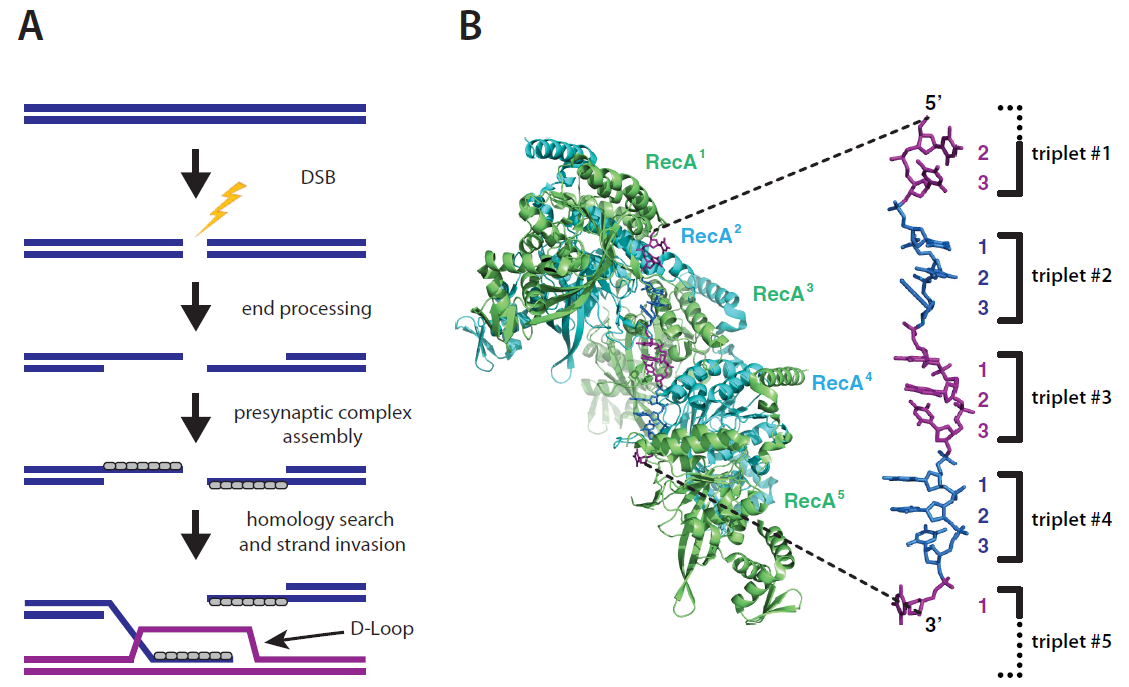
\includegraphics[width=0.5\linewidth]{3_1}
	\caption{А. Схематическое изображение первых стадий гомологической рекомбинации. Б. Кристаллическая структура RecA-ssDNA, которая показывает, как они связываются с триплетами(похожими на B форму, но не такими именно), образуя пресинаптический комплекс.}
	\label{fig:3_1}
\end{figure}

Про картинку \ref{fig:3_1}  (А). Там ебнешься это все расписывать, поэтому суть простая: ДНК рвется подлетаю друзья-белки образуют пресинаптический комплекс, затем появляется вторая молекула, они ищут в ней нужную гомологию и образуют D-loop(залуп), из которого и начинают синтез нужной последовательности

\begin{figure}[H]
	\centering
	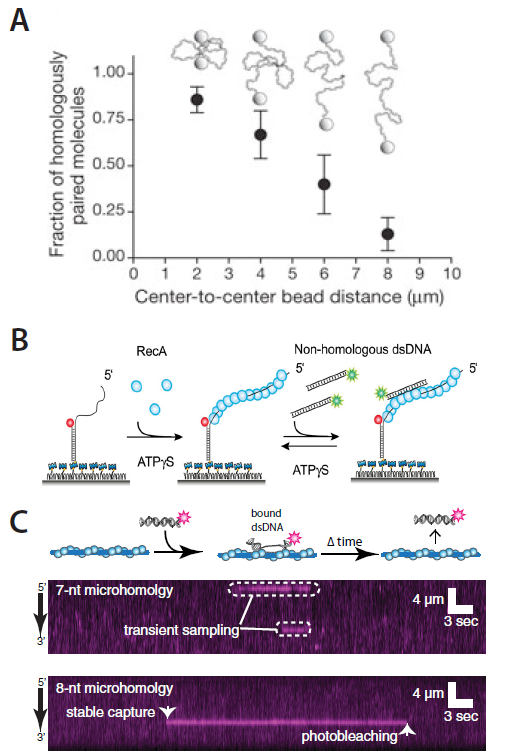
\includegraphics[width=0.5\linewidth]{3_2}
	\caption{А: График зависимости доли найденных гомологический спаренных молекул от расстояния между концами(подтверждающее, что гомологический поиск идет лучше для более спутанных молекул). Б: Картинка эксперимента по FRET (резонансная фотоскопия) исследованию гомологического поиска. В: Эксперимент показывающий, что переходное связывание найдено для ДНК с фрагментами, которые содержат меньше семи нуклеотидов в микрогомологии, а абсолютно стабильными являются фрагментами с 8ю нуклеотидами (стабильность аж до выцветания флюрофора)}
	\label{fig:3_2}
\end{figure}

Про картинку \ref{fig:3_2} (Б). Пресинпатические комплекс красились красными флюороформ, сам дуплекс красился зеленым, потом начинался процесс (запускали белок RecA) и потом запускались негомологические двунитевые молекулы ДНК. Когда два флюрофора приближались возникало свечение(он ссал в уши какой-то нефизичный бред). И дальше пихая туда разные ДНК получались зависимости частоты начала гомологической рекомбинации.

\begin{figure}[H]
	\centering
	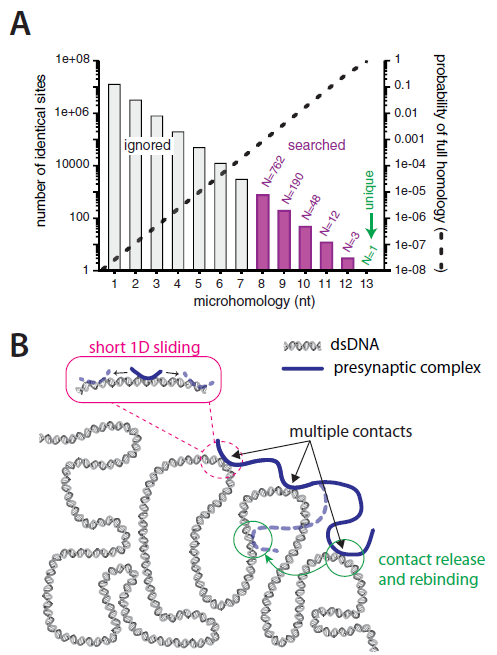
\includegraphics[width=0.5\linewidth]{3_3}
	\caption{А: Схематическая зависимость вероятности гомологического поиска от числа нуклеотидов внутри микрогомологии. Схематичное изображение основных принципов гомологического поиска: 1) одномерный сайдинг (скоростное (диффузионное?) скольжение в поисках нужных микрогомологий (розовый цвет), многоконтактность (синий цвет) и те самые интергементальные переходы (зеленый).}
	\label{fig:3_3}
\end{figure}

Про картинку \ref{fig:3_3} (А). Оказывается, что последовательности длинной меньше, чем 7 нуклеотидов, которые встречаются чаще (левая ось ординат), игнорируются при гомологическом поиске, а последовательность 8 и больше находятся, но очевидно, что вероятность полногот гомологического совпадения падает с увеличением длины микрогомологии.

\begin{figure}[H]
	\centering
	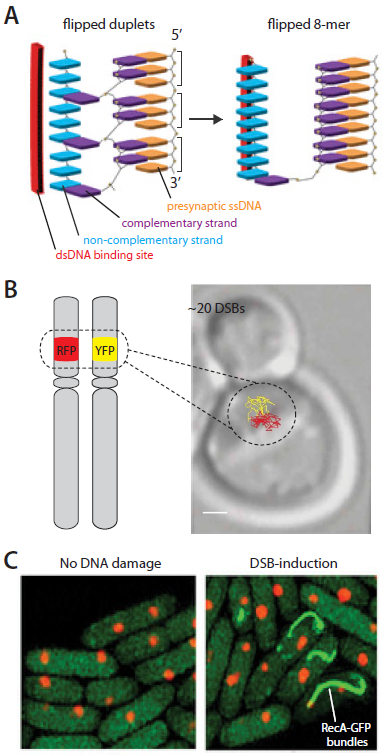
\includegraphics[width=0.5\linewidth]{3_4}
	\caption{А: Схематическое изображение взаимодействий дуплетов с образованием более устойчивых, связанных конфигураций. Б: Демонстрация диффузионного характера движения хромосом. В: С помощью флюоресценции показывается, что в поврежденном ДНК образуются RecA, которые ответственны за гомологическую рекомбинацию (зеленые) ВАУ!}
	\label{fig:3_4}
\end{figure}